\chapter{Inleiding}
\label{inleiding}
%In dit hoofdstuk wordt het werk ingeleid. Het doel wordt gedefinieerd en er
%wordt uitgelegd wat de te volgen weg is (beter bekend als de rode draad).
Het doel van deze masterproef is het ontwikkelen van een systeem dat in staat is om automatisch afbeeldingen te beschrijven. Dit probleem combineert twee domeinen uit de computerwetenschappen: enerzijds computervisie en anderzijds natuurlijke taalverwerking. Concreet moet het ontworpen systeem ongeziene afbeeldingen kunnen omzetten tot vloeiende, grammaticaal correcte Engelstalige zinnen. Bovendien moeten deze zinnen een zo volledig mogelijke omschrijving van de afbeelding vormen. Een voorbeeld van dergelijke afbeelding samen met een automatisch gegenereerde beschrijving is te zien in figuur \ref{fig:example_img}. Het concrete doel bestaat erin een bestaand systeem uit te breiden en te verbeteren. Hoofdstuk \ref{chap:Probleembeschrijving} gaat dieper in op deze doelstelling en licht de meest frequent gebruikte datasets voor training en evaluatie van beschrijvingssystemen toe.

\begin{figure}[tb]
    \centering
    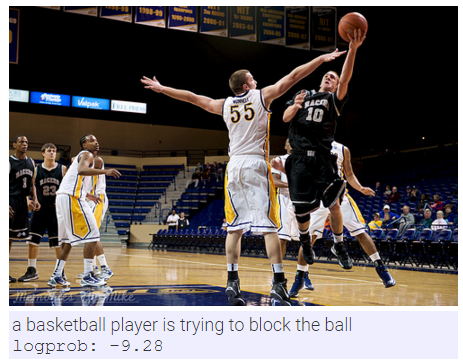
\includegraphics[width=0.65\textwidth]{Images/Results/Perfect/blocking_the_ball}
    \caption{Afbeelding met automatisch gegenereerde beschrijving}
    \label{fig:example_img}
\end{figure}

Om een beter inzicht te krijgen in het probleem en de mogelijke oplossingen, biedt hoofdstuk \ref{hoofdstuk:related} een uitgebreide literatuurstudie. Deze studie bekijkt relevante werken uit de computervisie en de natuurlijke taalverwerking. Daarnaast ligt de focus voornamelijk op recente onderzoeken die een soortgelijk doel als deze masterproef nastreven. Hieruit volgt een vergelijking van hoe deze papers afbeeldingen en zinnen voorstellen. Vervolgens onderzoekt de literatuurstudie op welke verschillende manieren deze representaties leiden tot een concreet systeem voor afbeeldingsbeschrijving.

Na de literatuurstudie volgt in hoofdstuk \ref{hst-theorie} een theoretische uitdieping van de concepten beschreven in de literatuurstudie. Een eerste sectie focust op neurale netwerken, die de basis vormen van het uiteindelijke systeem. Daarna volgt een uitdieping van twee statistische concepten die helpen bij het extraheren van zinvolle informatie uit afbeeldingen.

Hoofdstuk \ref{hst-meth} bespreekt de gebruikte methodologie om het afbeeldingsbeschrijvingsprobleem op te lossen. Een eerste sectie focust op een onderzoek (en bijhorende implementatie) uit de literatuurstudie die het basiswerk van deze masterproef vormt. Het doel van deze thesis is het verbeteren van de resultaten van dit referentiewerk. Het hoofdstuk start dan ook met een uitgebreide bespreking van het startpunt. Daarna volgt een beschrijving van eigen uitbreidingen van deze implementatie. Deze uitbreidingen behandelen nieuwe datasets, andere types neurale netwerken, verschillende vormen van extra semantische informatie en een vorm van normalisatie voor het genereren van de nieuwe zinnen. 

Om de verschillende uitbreidingen te kunnen vergelijken met het startpunt en modellen uit de literatuur, moet er een uniforme manier zijn om te evalueren. Menselijke evaluatie is hiervoor de ideale oplossing, maar dit is praktisch onhaalbaar. Om die reden bestaan er verschillende methodes om een getraind systeem te beoordelen. Hoofdstuk \ref{hoofdstuk:evaluatie} biedt een overzicht van automatische evaluatiemethodes uit de literatuur, alsook een aantal nieuwe evaluatiecriteria die de performantie van verschillende systemen vergelijken.

Het volgende hoofdstuk bespreekt de uitgevoerde experimenten in detail. Dit bevat onder andere de configuraties van de netwerken en hun uitbreidingen. Deze experimenten gaan na wat de invloed is van het toevoegen van verschillende vormen van semantische informatie en het type van netwerk. Daarnaast bespreekt het een tweede type van experiment, dat de ruisgevoeligheid van twee systemen nagaat.

Hoofdstuk \ref{cha:experimenten} bevat een uitvoerige bespreking van de uitgevoerde experimenten. Het biedt een overzicht van de configuraties van de verschillende netwerken en hun uitbreidingen. Naast de experimenten gerelateerd aan het genereren van nieuwe zinnen, beschrijft dit hoofdstuk ook een tweede type experiment, dat twee systemen vergelijkt in hun gevoeligheid voor onzuivere datasets.

In hoofdstuk \ref{cha:resultaten} volgt een uitvoerige bespreking van de resultaten van de eerder beschreven experimenten. Dit hoofdstuk bevat ook een vergelijking van de eigen systemen met de best presterende werken uit de literatuur.

Hoofdstuk \ref{besluit} sluit onze bijdrage met een overzicht van de conclusies die gemaakt zijn doorheen de masterproef.
 
%%% Local Variables:
%%% mode: latex
%%% TeX-master: "masterproef"
%%% End:
